\documentclass[a4paper,12pt]{report} % размер бумаги устанавливаем А4, шрифт 12 пунктов
\usepackage[T2A]{fontenc} % поддержка кириллицы в ЛаТеХ
\usepackage[utf8]{inputenc} % настройка кодировки
\usepackage[english,russian]{babel} % Определение языков в документе
\usepackage{amssymb,amsfonts,amsmath,mathtext,cite,enumerate,float} % подключаем нужные пакеты расширений
\usepackage{indentfirst} % делать отступ в начале параграфа
\usepackage{tabularx} % продвинутые таблицы
% \usepackage{showkeys} % раскомментировать, чтобы в документе были видны ссылки на литературу, рисунки и таблицы
\usepackage[labelsep=period]{caption} % заменить умолчальное разделение ':' на '.' в подписях к рисункам и таблицам
\usepackage[onehalfspacing]{setspace} % "умное" расстояние между строк - установить 1.5 интервала от нормального
\usepackage[final]{graphicx} % разрешить включение PostScript-графики
\graphicspath{{img/}} % Относительный путь к каталогу с рисунками

\usepackage{textcomp}
\newcommand*{\No}{\textnumero}

\makeatletter
\bibliographystyle{unstr} % Стиль библиографических ссылок БибТеХа - нумеровать в порядке упоминания в тексте
\renewcommand{\@biblabel}[1]{#1.} % Заменяем библиографию с квадратных скобок на точку в списке литературы
\makeatother

\def\labelitemi{--} % установка префикса немаркированного списка

% Настройка геометрии
\usepackage{geometry}
\geometry{left=2cm}
\geometry{right=1.5cm}
\geometry{top=1cm}
\geometry{bottom=2cm}

% настройка листинга
\usepackage{color} %% это для отображения цвета в коде
\usepackage{xcolor}
\usepackage{listings} %% собственно, это и есть пакет listings

\usepackage{hyperref}
\usepackage{multirow}
\usepackage{enumitem}

\DeclareCaptionFont{white}{\color{white}} %% это сделает текст заголовка белым
%% код ниже нарисует серую рамочку вокруг заголовка кода.
\DeclareCaptionFormat{listing}{\colorbox{gray}{\parbox{\textwidth}{#1#2#3}}}
\captionsetup[lstlisting]{format=listing,labelfont=white,textfont=white}
\lstset{ %
language=C, % выбор языка для подсветки (здесь это С)
basicstyle=\small\sffamily, % размер и начертание шрифта для подсветки кода
numbers=left, % где поставить нумерацию строк (слева\справа)
%numberstyle=\tiny, % размер шрифта для номеров строк
stepnumber=1, % размер шага между двумя номерами строк
numbersep=5pt, % как далеко отстоят номера строк от подсвечиваемого кода
backgroundcolor=\color{white}, % цвет фона подсветки - используем \usepackage{color}
showspaces=false, % показывать или нет пробелы специальными отступами
showstringspaces=false, % показывать или нет пробелы в строках
showtabs=false, % показывать или нет табуляцию в строках
frame=single, % рисовать рамку вокруг кода
tabsize=2, % размер табуляции по умолчанию равен 2 пробелам
captionpos=t, % позиция заголовка вверху [t] или внизу [b]
breaklines=true, % автоматически переносить строки (да\нет)
breakatwhitespace=false, % переносить строки только если есть пробел
escapeinside={\%*}{*)} % если нужно добавить комментарии в коде
}

% Меняем везде перечисления на цифра.цифра
\renewcommand{\theenumi}{\arabic{enumi}}
\renewcommand{\labelenumi}{\arabic{enumi}}
\renewcommand{\theenumii}{\arabic{enumii}}
\renewcommand{\labelenumii}{\arabic{enumi}.\arabic{enumii}.}
\renewcommand{\theenumiii}{\arabic{enumiii}}
\renewcommand{\labelenumiii}{\arabic{enumi}.\arabic{enumii}.\arabic{enumiii}.}

\renewcommand{\thesection}{\arabic{section}.}
% \renewcommand{\thesubsection}{\arabic{section}.\arabic{subsection}.}
\renewcommand{\thesubsection}{\arabic{subsection}.}
% \renewcommand{\thesubsubsection}{\arabic{section}.\arabic{subsection}.\arabic{subsubsection}.}
\renewcommand{\thesubsubsection}{\arabic{subsection}.\arabic{subsubsection}.}

\newtheorem{theorem}{Theorem}

\begin{document}
\def\figurename{Figure} % префикс к рисунками
\def\tablename{Table}
\newpage
\begin{titlepage}

\begin{center}\large{
    FEDERAL STATE AUTONOMOUS EDUCATIONAL INSTITUTION \\
    OF HIGHER EDUCATION \\*
    ITMO UNIVERSITY \\*
}\end{center}

\vspace{12em}

\begin{center}\large{
    Report \\
    on the practical task No. 6 \\
    <<Algorithms on graphs.
    Path search algorithms on weighted graphs>>
}\end{center}

\vspace{8.5em}

\flushright{Performed by}
\flushright{Sultan Zhumabaev}
\flushright{J4133c}
\vspace{1.5em}
\flushright{Accepted by}
\flushright{Dr Petr Chunaev}

\vspace{\fill}

\begin{center}
    St. Petersburg \\
    2020
\end{center}

\end{titlepage}

% \tableofcontents
\newpage
\subsection{Goal}\label{subsec:goal}

The use of path search algorithms on weighted graphs (Dijkstra's, A* and Bellman-Ford algorithms)

\subsection{Formulation of the problem}\label{subsec:formulation-of-the-problem}

\paragraph{I.} Generate a random adjacency matrix for a simple undirected weighted graph of 100 vertices and 500 edges with assigned random positive integer weights (note that the matrix should be symmetric and contain only 0s and weights as elements).
Use Dijkstra's and Bellman-Ford algorithms to find shortest paths between a random starting vertex and other vertices.
Measure the time required to find the paths for each algorithm.
Repeat the experiment 10 times for the same starting vertex and calculate the average time required for the paths search of each algorithm.
Analyse the results obtained.

\paragraph{II.} Generate a $10\times 10$ cell grid with 30 obstacle cells.
Choose two random non-obstacle cells and find a shortest path between them using A* algorithm.
Repeat the experiment 5 times with different random pair of cells.
Analyse the results obtained

\paragraph{III.} Describe the data structures and design techniques used within the algorithms.

\subsection{Brief theoretical part}\label{subsec:brief-theoretical-part}

A graph with no loops and no parallel edges is called a \textit{simple graph}.

\textit{Undirected graph} it is $G = (V, E)$, consisting of the set $V$ of nodes and the set $E$ of edges, which are unordered pairs of elements of $V$.

If edges in your graph have weights then your graph is said to be a \textit{weighted graph}, if the edges do not have weights, the graph is said to be \textit{unweighted}.

\textit{Dijkstra's Algorithm} (DA) is an algorithm for computing the shortest path between two vertices of a graph where all edges have nonnegative weight.
It is based on repeatedly expanding the closest vertex which has not yet been reached.
The complexity of the algorithm is estimated from $O(\lvert V \rvert \log{\lvert V \rvert})$ to $O(\lvert V \rvert^2)$, depending on the modification used.
This algorithm belongs to the class of greedy algorithms

The \textit{Bellman-Ford algorithm} (BFA) is an algorithm for computing the shortest path between two points in a weighted graph.
Unlike with \textit{Dijkstra's algorithm}, the edge weights are allowed to be negative.
On the down side, it has a larger running time, $O(\lvert V \rvert \lvert E \rvert)$.
This algorithm is related to Dynamic Programming Problems.

\textit{A*} search is a search algorithm which makes use of a heuristic which estimates the distance from a node to a goal state.
It iteratively expands nodes in order by their path cost plus their heuristic value.
If the heuristic satisfies certain "admissibility" conditions, then \textit{A*} is guaranteed to find an optimal path.
The time complexity of the algorithm is $O(\lvert E \rvert)$.
note that the algorithm \textit{A*} yields \textit{DA} if the heuristic is omitted.
This algorithm belongs to the class of greedy algorithms

\subsection{Results}\label{subsec:results}

Empirical comparison of the running time of algorithms \textit{DA} and \textit{BFA}:

\begin{verbatim}
    Dijkstra: 0.232 | Bellman-Ford: 0.843 | ration: 3.638
\end{verbatim}

\textit{Dijkstra's algorithm} is better when it comes to reducing the time complexity.
However, when we have negative weights, we have to go with the \textit{Bellman-Ford algorithm}.
Also, if we want to know whether the graph contains negative cycles or not, the \textit{Bellman-Ford algorithm} can help us with that.

Just one thing to remember, in case of negative weights or even negative cycles, the \textit{Bellman-Ford algorithm} can only help us with directed graphs.

The Figure~\ref{ris:plot} shows examples of the A* algorithm for finding the shortest distance for different pairs of vertices:

\begin{figure}[H]
    \center
    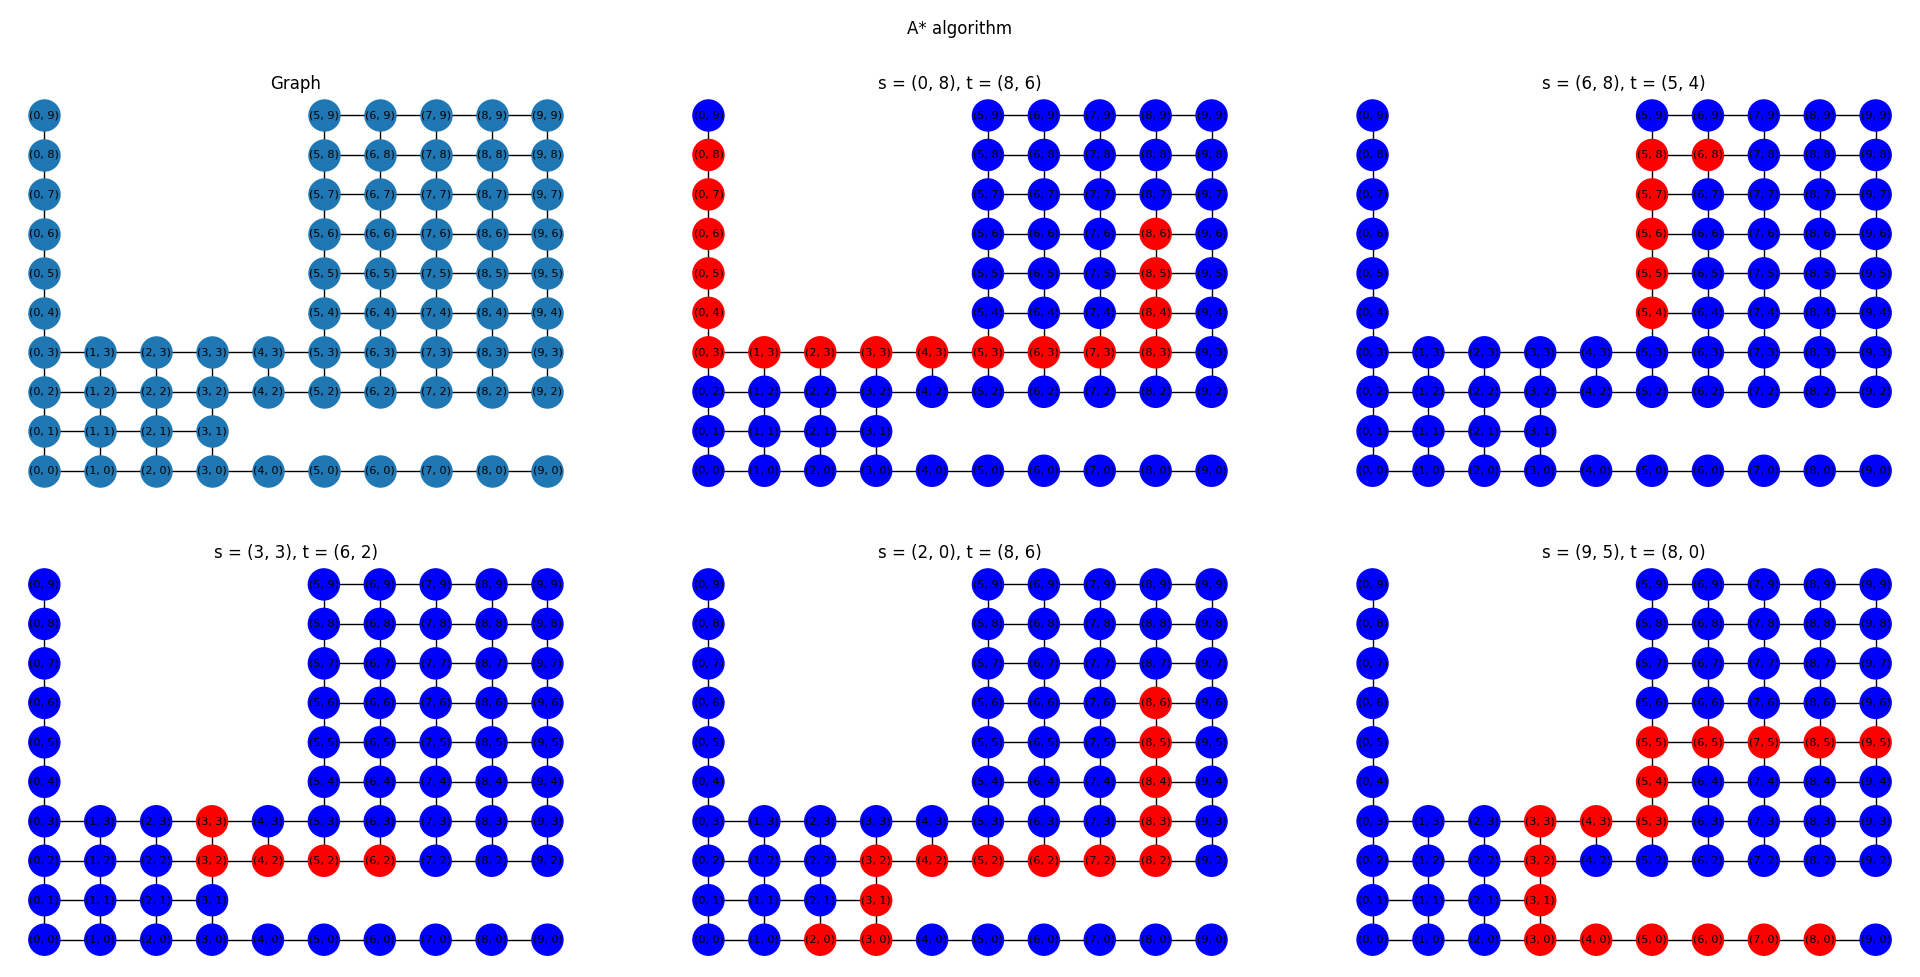
\includegraphics[width=\textwidth]{img/plot.png}
    \caption{Example of A* algorithm.}
    \label{ris:plot}
\end{figure}

If the heuristic gives an estimate of the shortest path from below (such a heuristic is called "acceptable"), then the A* search algorithm finds the shortest path.
In particular, the heuristic can always return 0.
in this case, the A* algorithm will be equivalent to the Dijkstra algorithm with a stop when the target vertex is reached.

If there is at least one path between the specified vertices in the graph, the A* algorithm always finds some path (regardless of the properties of the heuristic), since it is a generalization of the breadth-first search algorithm.

\subsection{Conclusion}\label{subsec:conclusion}

In this task, we applied and analyzed path-finding algorithms on weighted graphs (Dijkstra's algorithm, A*, and the Bellman-Ford algorithm).

\subsection{Appendix}\label{subsec:appendix}

The source code is located \href{https://github.com/vanSultan/anal_dev_algo/tree/lab_06}{here}: \url{https://github.com/vanSultan/anal_dev_algo/tree/lab_06}.

\end{document}
